\chapter{\ifproject%
\ifcpe โครงสร้างและขั้นตอนการทำงาน\else Project Structure and Methodology\fi
\else%
\ifcpe โครงสร้างของโครงงาน\else Project Structure\fi
\fi
}

ในบทนี้จะกล่าวถึงหลักการทำงาน และการออกแบบระบบของการเขียนบทความและการรีวิวกาแฟ

\makeatletter

% \renewcommand\section{\@startsection {section}{1}{\z@}%
%                                    {13.5ex \@plus -1ex \@minus -.2ex}%
%                                    {2.3ex \@plus.2ex}%
%                                    {\normalfont\large\bfseries}}

\makeatother
%\vspace{2ex}
% \titleformat{\section}{\normalfont\bfseries}{\thesection}{1em}{}
% \titlespacing*{\section}{0pt}{10ex}{0pt}

\section{การใช้งานของระบบ}
Usecase diagram ซึ่งเป็นการแสดงภาพรวมของการใช้งานของระบบ โดยจะแบ่งผู้ใช้งานเป็นสองกลุ่มคือ กลุ่มผู้เขียนบทความและรีวิว และกลุ่มผู้อ่านบทความ ซึ่งผู้ใช้ทั้งสองฝั่งจะใช้งานผ่านเว็บไซต์ Coffee blog 

\begin{figure}[h]
\begin{center}
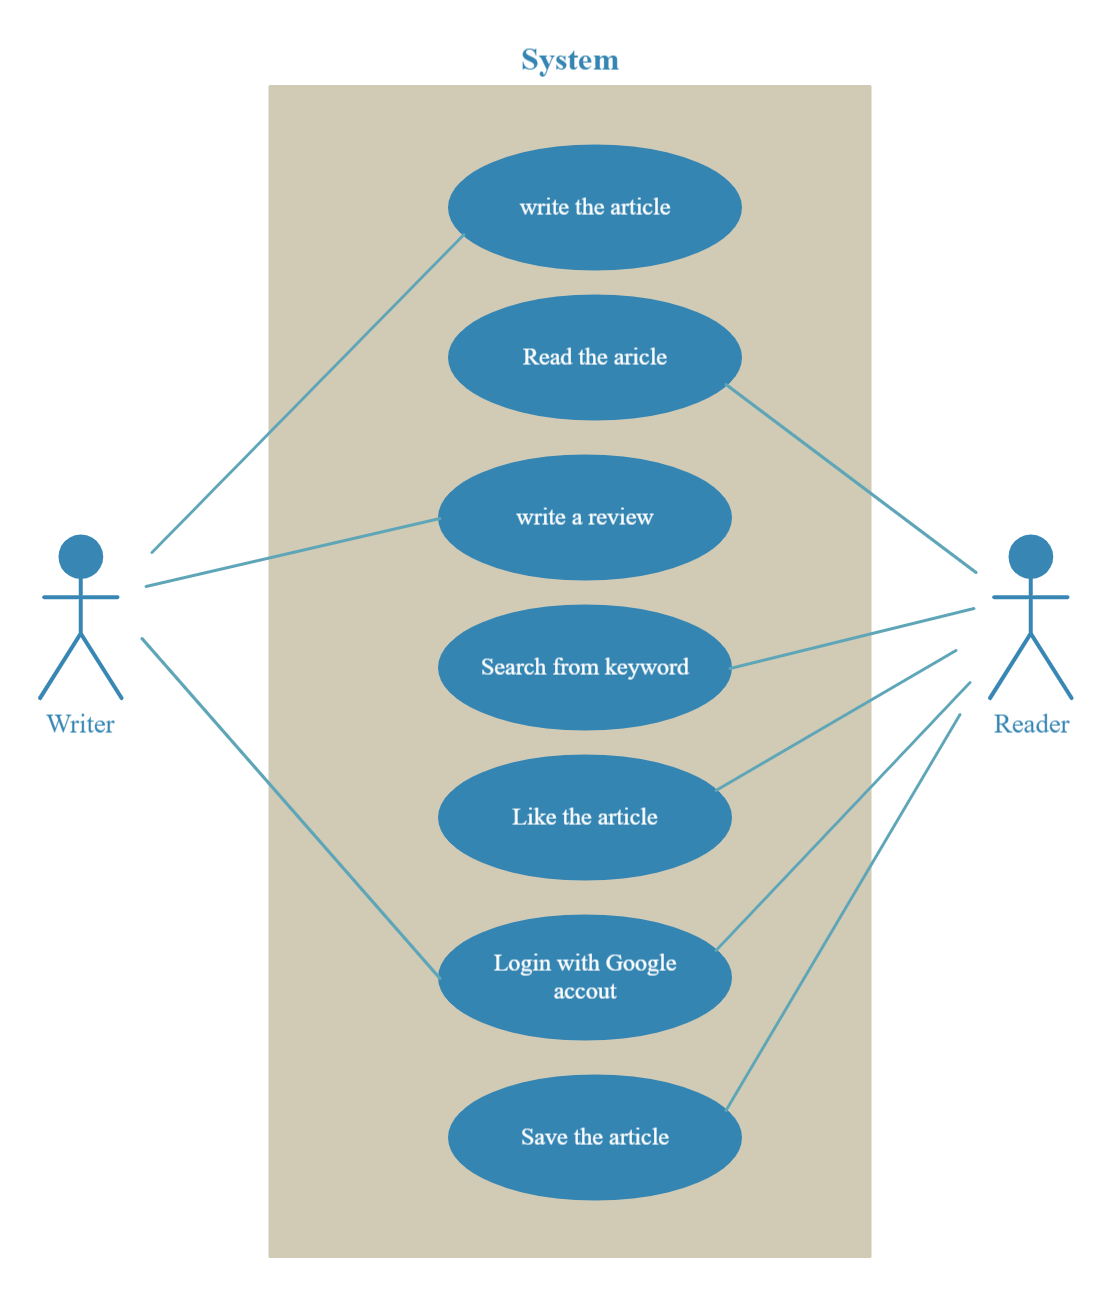
\includegraphics[width=6cm, height=8cm]{usecase-diagram.jpg}
\end{center}
\caption[Usecase diagram]{usecase diagram ของระบบ}
\end{figure}

การใช้งานของระบบจะมีการทำงานดังตัวอย่างต่อไปนี้ \\ 
Use case 1 \\ 
Usecase Title : การเขียนบทความ\\
Primary Actor : ผู้เขียนบทความ\\
Stakeholder Actor : ผู้อ่านบทความ\\
Main Flow : ผู้ใช้ทั้งสองฝั่งเข้าสู่ระบบด้วย Google account ผู้ที่เขียนบทความเข้าไปเขียนบทความในหน้าบทความ และกดโพสต์บทความเพื่อทำการสร้างบทความ และเลือก tag สำหรับบทความเพื่อให้ผู้ที่เข้ามาอ่านสามารถค้นหาบทความได้ง่ายขึ้น\\
Exceptional Flow : เมื่อเขียนบทความเสร็จ ผู้อ่านจะสามารถเข้ามาอ่านได้ ยอดการเข้าอ่านบทความจะเพิ่มขึ้น\\ \\
Use case 2 \\
Usecase Title : การอ่านบทความ\\
Primary Actor : ผู้อ่านบทความ\\
 Stakeholder Actor : ผู้เขียนบทความ\\
Main Flow : ผู้ใช้ทั้งสองฝั่งเข้าสู่ระบบด้วย Google account ในหน้าแรกผู้ใช้สามารถค้นหา keyword ที่ต้องการเข้าไปอ่านได้ ถ้าผู้ใช้ชอบบทความที่เข้าไปอ่านผู้ใช้สามารถ like บทความ และ save ไว้อ่านทีหลังได้\\
 Exceptional Flow : เมื่อกด save บทความผู้ใช้จะสามารถเข้าไปดูบทความที่ save ได้\\ \\
Use case 3\\
Usecase Title : การเขียนรีวิว\\
Primary Actor : ผู้เขียนรีวิว\\
 Stakeholder Actor : ผู้อ่านรีวิว\\
Main Flow : ผู้ที่ต้องการเขียนรีวิว จะถ่ายรูปกาแฟ หรือถุงกาแฟที่ตนเองต้องการรีวิว และอัพโหลดไปที่เว็บไซต์ เขียนรายระเอียดเกี่ยวกับกาแฟ และเลือกสีที่ต้องการ \\
 Exceptional Flow : เมื่อเขียนรีวิวเสร็จ ผลลัพธ์ที่ได้จะได้เป็นหน้าแสดงผล เช่นกราฟ และสรุปของสี ที่เกี่ยวกับกาแฟ\\

 \section{โครงสร้างของระบบ}
 โดยภาพรวมของระบบจะเป็นดังภาพ ซึ่งในส่วนของผู้ใช้ หรือ client จะใช้ React Next.js ในการพัฒนา และมีตัวกลางในการติดต่อเรียกใช้ข้อมูลระหว่าง server กับ client คือ GraphQL และในส่วนของ server จะใช้ Nodejs ในการพัฒนา ฐานข้อมูล จะมีสองส่วน คือ Elasticsearch จะทำในส่วนของการเก็บข้อมูลที่ใช้ในการ search และ MongoDB ที่จะเก็บข้อมูลต่างๆ
\begin{figure}[h]
\begin{center}
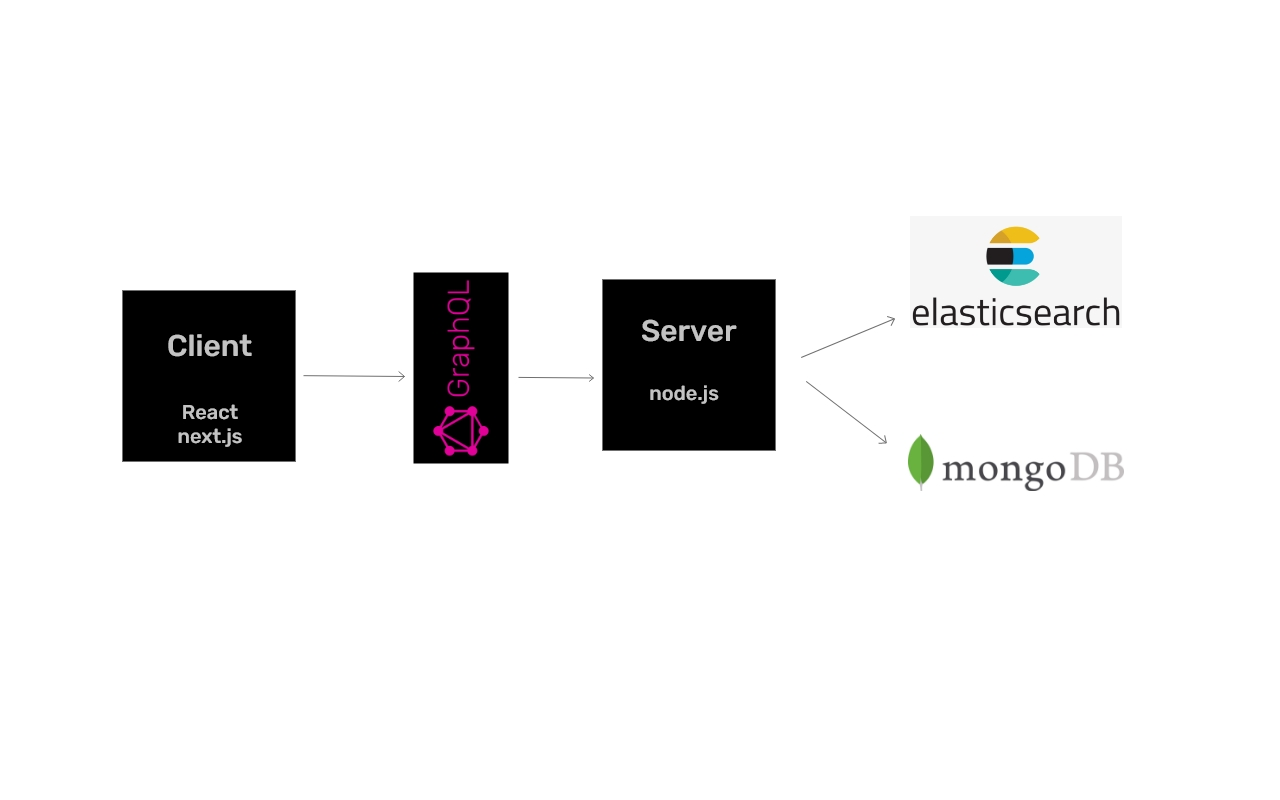
\includegraphics[width=10cm, height=8cm]{database.jpg}
\end{center}
\caption[Application Model]{แผนผังการทำงานของระบบ}
\end{figure}
หลักการทำงานของระบบ
\begin{enumerate}
  \item ผู้ใช้สามารถเข้าเว็บไซต์ได้จากสมาร์ทโฟน แท็บเล็ต หรือคอมพิวเตอร์
  \item เมื่อผู้ใช้ต้องการค้นหาบทความจะเรียกของมูลมาจาก elasticsearch โดยใช้ graphql เป็นตัวกลางในการเรียกใช้ข้อมูล
  \item เมื่อผู้ใช้ต้องการเขียนบทความหรือเขียนรีวิว ข้อมูลจะอัพเดตและเก็บไว้ใน MongoDB 
  \item การทำงานของผู้ใช้ทั้งหมดจะสามารถใช้งานบนเว็บไซต์ทั้งหมด
\end{enumerate}
สาเหตุที่ทำเว็บไซต์เพื่อให้ผู้ใช้สามารถเข้าถึงได้ในอุปกรณ์ต่างๆ และมีความง่ายต่อการพัฒนา
